\documentclass[a4paper,11pt]{article}
\usepackage{amsmath,amsthm,amsfonts,amssymb,amscd,amstext,vmargin,graphics,graphicx,tabularx,multicol} 
\usepackage[francais]{babel}
\usepackage[utf8]{inputenc}  
\usepackage[T1]{fontenc} 
\usepackage{pstricks-add,tikz,tkz-tab,variations}
\usepackage[autolanguage,np]{numprint} 

\setmarginsrb{1.5cm}{0.5cm}{1cm}{0.5cm}{0cm}{0cm}{0cm}{0cm} %Gauche, haut, droite, haut
\newcounter{numexo}
\newcommand{\exo}[1]{\stepcounter{numexo}\noindent{\bf Exercice~\thenumexo} : \marginpar{\hfill /#1}}
\reversemarginpar


\newcounter{enumtabi}
\newcounter{enumtaba}
\newcommand{\q}{\stepcounter{enumtabi} \theenumtabi.  }
\newcommand{\qa}{\stepcounter{enumtaba} (\alph{enumtaba}) }
\newcommand{\initq}{\setcounter{enumtabi}{0}}
\newcommand{\initqa}{\setcounter{enumtaba}{0}}

\newcommand{\be}{\begin{enumerate}}
\newcommand{\ee}{\end{enumerate}}
\newcommand{\bi}{\begin{itemize}}
\newcommand{\ei}{\end{itemize}}
\newcommand{\bp}{\begin{pspicture*}}
\newcommand{\ep}{\end{pspicture*}}
\newcommand{\bt}{\begin{tabular}}
\newcommand{\et}{\end{tabular}}
\renewcommand{\tabularxcolumn}[1]{>{\centering}m{#1}} %(colonne m{} centrée, au lieu de p par défault) 
\newcommand{\tnl}{\tabularnewline}

\newcommand{\bmul}[1]{\begin{multicols}{#1}}
\newcommand{\emul}{\end{multicols}}

\newcommand{\trait}{\noindent \rule{\linewidth}{0.2mm}}
\newcommand{\hs}[1]{\hspace{#1}}
\newcommand{\vs}[1]{\vspace{#1}}

\newcommand{\N}{\mathbb{N}}
\newcommand{\Z}{\mathbb{Z}}
\newcommand{\R}{\mathbb{R}}
\newcommand{\C}{\mathbb{C}}
\newcommand{\Dcal}{\mathcal{D}}
\newcommand{\Ccal}{\mathcal{C}}
\newcommand{\mc}{\mathcal}

\newcommand{\vect}[1]{\overrightarrow{#1}}
\newcommand{\ds}{\displaystyle}
\newcommand{\eq}{\quad \Leftrightarrow \quad}
\newcommand{\vecti}{\vec{\imath}}
\newcommand{\vectj}{\vec{\jmath}}
\newcommand{\Oij}{(O;\vec{\imath}, \vec{\jmath})}
\newcommand{\OIJ}{(O;I,J)}


\newcommand{\reponse}[1][1]{%
\multido{}{#1}{\makebox[\linewidth]{\rule[0pt]{0pt}{20pt}\dotfill}
}}

\newcommand{\titre}[5] 
% #1: titre #2: haut gauche #3: bas gauche #4: haut droite #5: bas droite
{
\noindent #2 \hfill #4 \\
#3 \hfill #5

\vspace{-1.6cm}

\begin{center}\rule{6cm}{0.5mm}\end{center}
\vspace{0.2cm}
\begin{center}{\large{\textbf{#1}}}\end{center}
\begin{center}\rule{6cm}{0.5mm}\end{center}
}



\begin{document}
\pagestyle{empty}
\titre{Interrogation: Multiplications }{Nom :}{Prénom :}{Classe}{Date}


\vspace*{0.5cm}
\begin{flushleft}
\begin{tabular}{|m{9.5cm}|m{1.25cm}|m{1.25cm}|m{1.25cm}|m{1.25cm}|m{1.25cm}|}
\hline 
\textbf{Compétences} & \begin{center}
\textbf{N.E.}
\end{center} & \begin{center}
\textbf{M.I.}
\end{center} & \begin{center}
\textbf{M.F.}
\end{center}  & \begin{center}
\textbf{M.S.}
\end{center} & \begin{center}
\textbf{T.B.M.}
\end{center} \\ 
\hline 
Je dois savoir multiplier des nombres décimaux (calcul mental ou posé) & & &  & &\\
\hline
Je dois savoir multiplier par 10, 100, 1000 etc& & &  & & \\ 
\hline
Je dois savoir multiplier par 0,1; 0,01 ; 0,001 etc & & &  & & \\ 
\hline 


\end{tabular}  
\end{flushleft}

\textit{N.E = Non évalué ; M.I. = Maîtrise insuffisante ; M.F. = Maîtrise fragile ; M.S. = Maîtrise satisfaisante ; T.B.M. = Très bonne maîtrise}\\



\exo{2} Poser et calculer les opérations suivantes :\\

$768 \times 345$ \hspace*{6cm} $3,91 \times 84,2$\\

\vspace*{7cm}

\exo{2.25} Compléter par le nombre manquant :\\

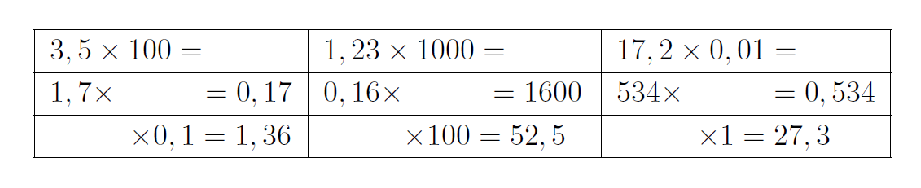
\includegraphics[scale=1.05]{multi.eps} \\




\exo{2} Calculer astucieusement les expressions suivantes :

\bmul{2}

$H = 2 \times 136,2 \times 500  $\\
\reponse[5]\\

\columnbreak

$M = 0,25  \times 9 \times 4 \times 8$\\
\reponse[5]\\

\emul

\newpage

\exo{1.5}  Dans la classe de Fanny, il y a quatre rangées de tables.\\ Par rangée, il y a 5 tables. \\
Par table, il y a deux chaises.\\
Combien y a-t-il de chaises dans cette salle de classe?\\
\reponse[6]\\


\exo{2.25} Dans une salle de cinéma, le prix d'une séance le matin est de 5,80 euros. \\
L'après-midi et le soir, la séance est à 9 euros.\\
Le cinéma propose également une carte "5 places" pour 35 euros valable pour n'importe quelle séance de cinéma.\\

\q \qa Coralie va toujours au cinéma avant midi. Combien paye-t-elle pour 5 séances de cinéma si elle ne choisit pas la carte.\\
\reponse[4]\\

\qa A-t-elle intérêt à acheter la carte "5 places" ? Justifier votre réponse.\\
\reponse[4]\\

\q Mathieu ne va au cinéma qu'en soirée. Pour lui, cela vaut-il la peine de choisir la carte "5 places" ? Justifier votre réponse.\\
\reponse[4]\\

\vspace*{1.5cm}

\exo{} BONUS\\

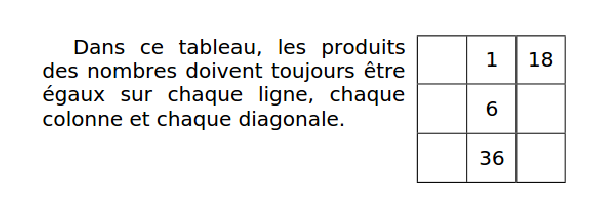
\includegraphics[scale=1.2]{carremagiquex.eps} 


\end{document}
